\section{Cloud Infrastruktur}

Das Trainieren eines \textit{Deep Learning} Modells ist gerade bei großen CNN Architekturen äußerst rechenaufwendig. Tensor Operationen wie Matrixmultiplikationen und Konvolutionen erfordern im Rahmen des maschinellen Lernens hohe Parallelisierung und Taktfrequenzen, um in absehbarer Zeit gute Ergebnisse zu liefern. Die Rechenkapazität normaler Desktop-PCs reicht demnach meist nicht aus, um performantes \textit{Deep Learning} betreiben zu können. 

Abhilfe bieten Software-as-a-Service (SaaS) bzw. Platform-as-a-Service (PaaS) Angebote wie \textit{Amazon SageMaker}, \textit{Google Cloud Platform Cloud AI} oder \textit{Azure ML Services} oder aber auch Start-ups wie \textit{FloydHub}. Diese bieten Infrastruktur in unterschiedlichen Zonen je nach Standpunkt der Rechenzentren zum Trainieren an sowie eine Plattform zum Verwalten der \textit{Deep Learning} Prozesse. 

\subsection*{Trainingshardware}

Gerade GPUs bieten sich aufgrund ihres hohen Parallelisierungsvermögens gegenüber herkömmlichen CPUs an. Insbesondere \textit{NVIDIA} nimmt hierbei eine Vorreiterrolle in der Produktion von Server-GPUs ein. Die \textit{Compute Unified Device Architecture} (CUDA) von \textit{NVIDIA} ermöglicht hierbei als Programmiermodel und parallele Computing Plattform das Auslagern von Rechenprozessen auf GPUs. Das \textit{CUDA} Toolkit beinhaltet GPU beschleunigte Bibliotheken, einen Compiler, Entwicklungswerkzeuge sowie die eigentliche \textit{CUDA} Laufzeit und wird von vielen \textit{Deep Learning} Bibliotheken genutzt, wie z.B. \textit{PyTorch} \cite{NVIDIA.20200209} \cite{PyTorch.20200209}. 

Vergleich man gängige Tesla GPUs, die Kunden als PaaS-Angebot zur Verfügung gestellt werden, nach ihrer Rechenleistung, so ergibt sich Tabelle \ref{gpus} \cite{TechPowerUp.20200209}.

\begin{center}
	\begin{tabular}[h]{l|c|c|c|c|c|c}
		& K80 & P100 & T4 & V100 & GTX 1080 & TITAN RTX \\
		\hline
		CUDA Cores & 2496 & 3584 & 2560 & 5120 & 2560 & 4608 \\
		Tensor Cores & / & / & 320 & 640 & / & 576 \\
		TeraFLOPS (Single Precision) & 4,113 & 9,526 & 8,141 & 14,13 & 8,873 & 16,31 \\
		Memory Bandwidth (in GB/sec) & 240,6 & 732,2 & 320 & 897 & 320,3 & 672 \\
		Suggested Power Supply Unit & 700 & 600 & 350 & 600 & 450 & 600
		\label{gpus}
	\end{tabular}
	\captionof{table}{Vergleich von GPUs nach Rechenleistung}
\end{center}

Auch wurde die \textit{GeForce GTX 1080} sowie die \textit{Titan RTX}, zwei Desktop-Grafikkarten ausgelegt auf Gaming und Entertainment, in den Vergleich mit aufgenommen. Der Vergleich dient später dazu, um eine begründete Kosten-Nutzen Abwägung zwischen einem Trainieren der Modelle auf der CLoud oder lokal vollziehen zu können.

Neben GPUs existieren seit 2015 die von Google entwickelten \textit{Tensor Processing Units} (TPUs). Diese Art von Spezialhardware erreicht pro TPU-Kern eine Rechenleistung von bis zu 92 TOPS \cite{HaraldBogeholz.20170406}. Schließt man 2048 solcher TPU-Kerne zu einem TPU-Pod zusammen, so ergibt sich eine Rechenleistung von über 100 PetaFLOPS \cite{GoogleCloud.20200209}. Zudem ist die größere Rechenleistung gleichzeitig effizienter als herkömmliche GPUs (siehe Abbildung \ref{tpu})

\begin{figure}[ht]
	\begin{center}
		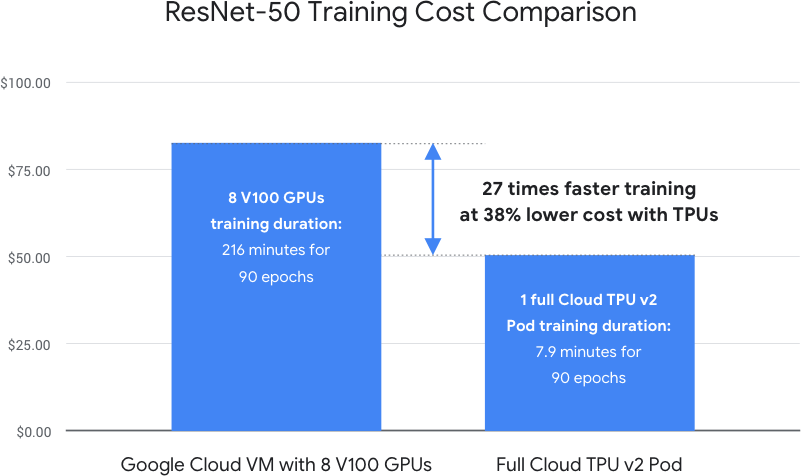
\includegraphics[width=14cm]{Bilder/tpu_comparison.png} 
		\caption[Vergleich V100 - TPU Pod]{Vergleich V100 - TPU Pod \cite{GoogleCloud.20200209b}}
		\label{tpu}
	\end{center}
\end{figure}

Eine weitere Steigerung versprechen Microsofts Field Programmable Gate Arrays (FPGAs), die allerdings nicht weiter im Rahmen dieser Arbeit betrachtet werden sollen \cite{KarlFreund.20170828}.

\subsection*{FloydHub}

FloydHub, ein kalifornisches Start-up, bietet eine Data-Science Plattform zum Trainieren und Bereitstellen von \textit{Deep Learning} Applikationen. FloydHub erlaubt es Anwendern sich auf reines \textit{Deep Learning} zu konzentrieren, während es die Arbeit rund um den \textit{Deep Learning} Lebenszyklus abnimmt. Hierzu gehört das Bereitstellen der entsprechenden Hardware, das Installieren von Treibern oder das Integrieren verschiedener \textit{Deep Learning} Bibliotheken, wie \textit{TensorFlow}, \textit{PyTorch} oder \textit{Keras} \cite{FloydHub.20200215}. 

Mit Hilfe des von FloydHub bereitgestellten Command Line Interfaces (CLI) kann ein lokales Projekt zu einem FloyHub Projekt initialisiert werden. Anschließend können anhand einer Konfigurationsdatei Einstellungen über das Training spezifiziert werden. Alternativ können diese auch über das CLI festgelegt werden. 

\lstset{language=XML}
\lstinputlisting[
label=floydhub:FloydHub,
caption=Konfigurationsdatei zum Trainingsjob,
captionpos=b,
firstline=1,
lastline=9
]{Quellcode/floyd.yml}

Hierbei kann zwischen der K80 (gpu) oder der V100 (gpu2) GPU für das Training gewählt werden. Auch die \textit{Deep Learning} Laufzeitumgebung muss spezifiziert werden. Bei Bedarf auch zusätzliche Bibliotheken in einer \textit{floyd\_requirements.txt}-Datei zur Installation mit angegeben werden. Anschließend muss der Datensatz referenziert werden, mit dem das Modell trainiert werden soll. 

Dieser Datensatz wird separat hochgeladen, da sich dieser im Gegensatz zum Programmcode nur selten ändert. FloydHub implementiert auf seiner Plattform eine Art Pfadsystem, unter dem Datensätze und Projekte abgespeichert werden. Diese Pfade werden in der Konfigurations-Datei zur Referenzierung genutzt. Um auch im Programmcode auf den Datensatz zuzugreifen, muss ein Mountname definiert werden. In obigen Beispiel wird dem Datensatz unter Verzeichnis \textit{<username>/datasets/smartwarehousessd/3} der Mountname \textit{ssd} gegeben. Das Verzeichnis zum Einlesen der Daten ist anschließend im Code unter \textit{/floyd/input/ssd/} erreichbar. 

Mit dem CLI Befehl \textit{floyd run} wird der Programm Code auf die Plattform hochgeladen und der in der Konfigurationsdatei angegebene Befehl ausgeführt. Daraufhin wird ein Job erstellt, versioniert und ausgeführt. Während der Job ausgeführt wird, wird dem Nutzer ein Einblick in die Konsolenausgabe gewährt sowie in Metriken zur Hardwareauslastung. In der Jobhistorie kann im Nachhinein jeder Job mit dem damals aktuellen Programmcode und Datensatz eingesehen werden. Auch Datensätze werden versioniert. Schreibrechte sind auf das Verzeichnis \textit{/floyd/home} begrenzt, hier können Zwischenspeicherpunkte des Modells abgelegt werden. 

FloydHub betreibt ein zeitbasiertes Zahlungsmodell. So kosten 10 Stunden Laufzeit auf einer K80 12\$, auf einer V100 bereits 42\$. Zusätzlich werden monatliche Account-Gebühren berechnet. Je nach Account kann eine unterschiedliche Anzahl an Projekten erstellt und Speicherplatz verwendet werden. Die \textit{Beginner} Ausstattung von einem Projekt und 10 GB Speicher ist allerdings kostenfrei. 
